\documentclass{article}
 \usepackage{tikz}
 \begin{document}
 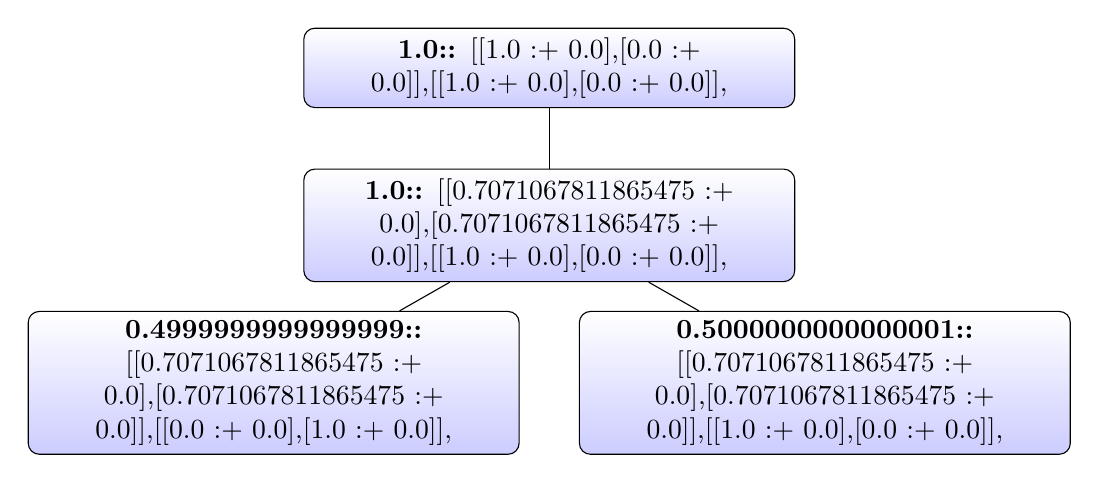
\begin{tikzpicture}[sibling distance=7cm,  every node/.style = {shape=rectangle, rounded corners,    draw, align=center,    top color=white, bottom color=blue!20}]]
  \node[text width=6cm]{ \textbf{1.0:: }[[1.0 :+ 0.0],[0.0 :+ 0.0]],[[1.0 :+ 0.0],[0.0 :+ 0.0]], } [level distance=2cm]
	child { node[text width=6cm]{ \textbf{1.0:: }[[0.7071067811865475 :+ 0.0],[0.7071067811865475 :+ 0.0]],[[1.0 :+ 0.0],[0.0 :+ 0.0]], } [level distance=2cm]
	child { node[text width=6cm] { \textbf{0.4999999999999999:: }[[0.7071067811865475 :+ 0.0],[0.7071067811865475 :+ 0.0]],[[0.0 :+ 0.0],[1.0 :+ 0.0]], } }
	child { node[text width=6cm] { \textbf{0.5000000000000001:: }[[0.7071067811865475 :+ 0.0],[0.7071067811865475 :+ 0.0]],[[1.0 :+ 0.0],[0.0 :+ 0.0]], } } };
\end{tikzpicture}

\begin{tabular}{|c|c|}
\hline
0.5000000000000001 & 0.4999999999999999 \\ 
00 & 10 \\ 
\hline
\end{tabular}

\begin{tabular}{|c|c|c|c|}
\hline
0.25 & 0.2499999999999999 & 0.2500000000000001 & 0.25 \\ 
01 & 11 & 00 & 10 \\ 
\hline
\end{tabular}

\end{document}